\section{Results}\label{sec:results}

As described in \autoref{sec:project}, the data of 5992 songs by German rap artists formed the basis of our research. For each song, information on the artists contributing, the album and the date of release was stored. This information was obtained using the Genius API. In addition, the final data set contains the lyrics to the corresponding song, which were treated using the preprocessing procedure described above and also saved in modified form.

The 5992 songs that remained after discarding non-German songs include 2094 participating artists and are spread among 1711 different albums. The number of artists involved includes not only primary artists, but also producers and featured artists. For example, the two producers Tim Wilke and David Kraft are the most frequent artists with 68 occurrences in the 5992 songs. The third most frequent artist in the available lyrics is Sido with 65 occurrences.

888 songs were declared as singles by Genius and were therefore not assigned to an album. This class also forms by far the largest share of the existing albums. The other existing albums are largely based on the limitation of song scraping to 15 songs per artist (see \autoref{sec:project}). The albums 'Instinkt' and 'Berlins Most Wanted' are both listed as 15 albums of one song. Only the album 'Liebeskummerparty' has 16 occurrences due to a song with a different artist.

\autoref{fig:number_songs} shows the temporal distribution of the songs. As it can be seen from the figure, the data set contains considerably fewer songs in the years 1998 to 2010 than in the period from 2010 to 2022. This could be due to the procedure for generating the data, which is essentially based on the predefined playlists from Spotify and the availability of various songs on the lyrics platform Genius. In addition, the number of artists in the Deutschrap genre has grown steadily over the years and was very low when the genre first emerged. The described disparity of the data affects the interpretability of the analyses. Details on this are explained in detail in the following sections.

\begin{figure}[!htb]
    \centering
    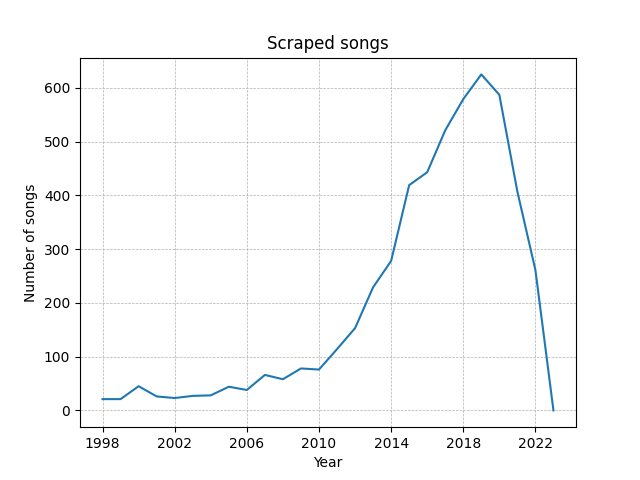
\includegraphics[width=0.8\textwidth]{figures/number_of_songs.png}
    \label{fig:number_songs}
    \caption{Temporal distribution of scraped songs}
\end{figure}

In the following, the results of the three different approaches to analyze the data will be presented in detail.

\subsection*{Occurrences check}

As outlined in \autoref*{sec:project}, an essential part of the task of the Occurrences Check was to elaborate a suitable dictionary for different categories, on the basis of which occurrences within the lyrics could be retrieved. After executing the process described in \autoref{sec:project} via Word2Vec and manual adjustment, the following quantities of words remained per category:

\def\arraystretch{1.2}
\begin{table}[!hbt]
    \centering
    \begin{tabular}{|l|l|}
    \hline
    \textbf{Category} & \textbf{Number of words} \\ \hline
    Misogyny        & 19 \\ \hline
    Violence        & 17 \\ \hline
    Anti-Semitism   & 14 \\ \hline
    Homophobia      & 14 \\ \hline
    Anti-disability & 13 \\ \hline
    Grief           & 12 \\ \hline
    Love            & 10 \\ \hline
    Racism          & 6  \\ \hline
    \end{tabular}
    \caption{Number of terms within each category of occurrences check}
    \label{tab:dictionary}
\end{table}

The different number of words per category is due to the fact that certain categories have fewer diverse terms than others. For example, the category misogyny contains a wide variety of vulgar terms for prostitutes, while the racism category almost exclusively contains the word 'nigger'.

The following \autoref{tab:occurrences_total} shows the absolute count of occurrences of the different categories in the entire data set. The categories love, misogyny and violence combine more than 85\% of all occurrences with 31451 of 36833 counted occurrences. 3628 of the examined songs contain at least one occurrence of the category love, which corresponds to about 61\% of the entire data set. The category violence was detected at least once in 3099 songs, approximately 52\% of all songs. We detected misogynistic terms in 2431 songs, about 41\% of the population. In 757 songs, no occurrences of the predefined categories could be found.

\begin{table}[!htb]
    \centering
    \begin{tabular}{|l|l|}
    \hline
    \textbf{Category} & \textbf{Number of occurrences} \\ \hline
    Love              & 12098                          \\ \hline
    Violence          & 10251                          \\ \hline
    Misogyny          & 9102                           \\ \hline
    Racism            & 2051                           \\ \hline
    Grief             & 1294                           \\ \hline
    Homophobia        & 1253                           \\ \hline
    Anti-disability   & 546                            \\ \hline
    Anti-semitism     & 238                            \\ \hline
    \end{tabular}
    \caption{Absolute count of occurrences of investigated categories}
    \label{tab:occurrences_total}
\end{table}

For further analysis, we examined the behaviour of the occurrences based on the release date of the songs. Due to the previously mentioned bias in the number of songs per year, we normalised the number of occurrences per year. \autoref{fig:occurrences_time_series} shows the development of the occurrences over the examined period 1998 to 2022. The different lines show the normalised number of occurrences per song for each category. The different categories are marked with different colours. It can be observed that especially around the year 2003, a relatively large number of songs contained violent and misogynistic terms, but at the same time also many on the subject of love. Until 2010, the occurrences of the three mentioned categories decrease to an average level of 3 occurrences per song. They maintain this level in the following years up to 2022. The other categories are less prevalent throughout the entire study period: Only the categories homophobia in 2006 and racism in 2003 exceed the mark of 1 average occurrence per song.

\subsection*{Sentiment analysis}



\subsection*{Zero-shot classifier}

\begin{figure}[!htb]
    \centering
    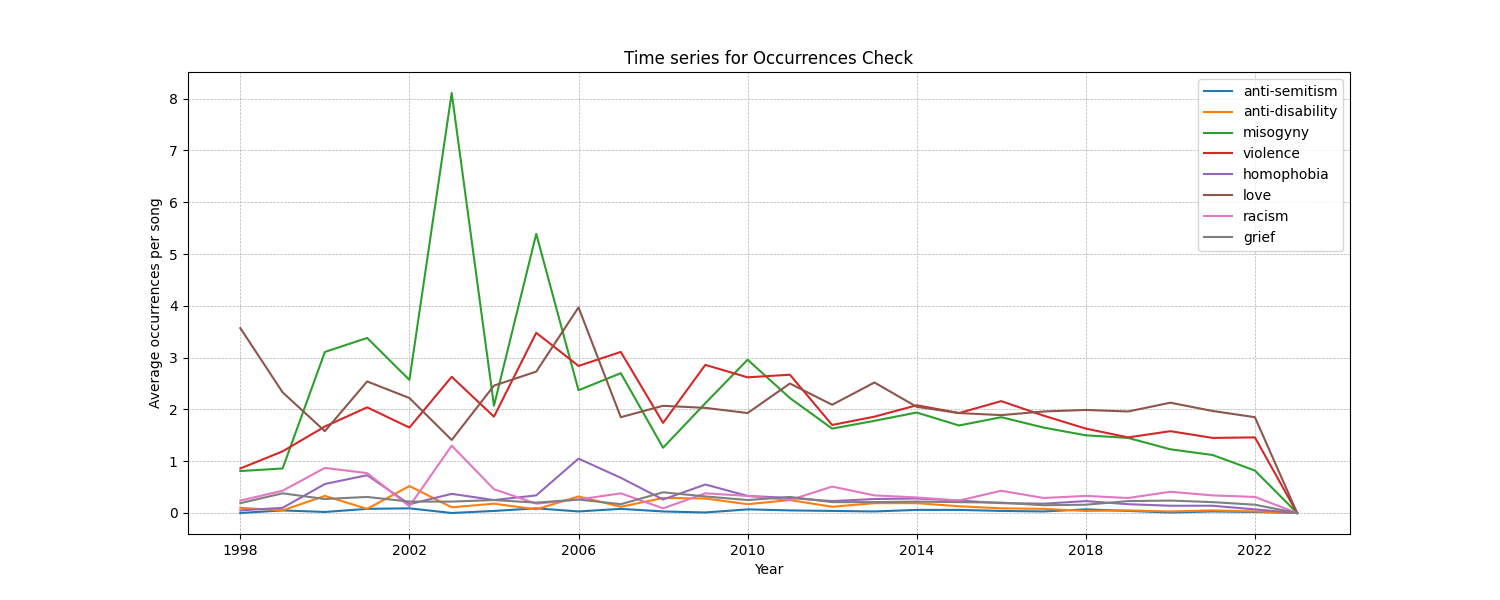
\includegraphics[width=\textwidth]{figures/time_series_occurrences.png}
    \caption{Time series analysis of counted occurrences}
    \label{fig:occurrences_time_series}
\end{figure}


\begin{figure}[!htb]
    \centering
    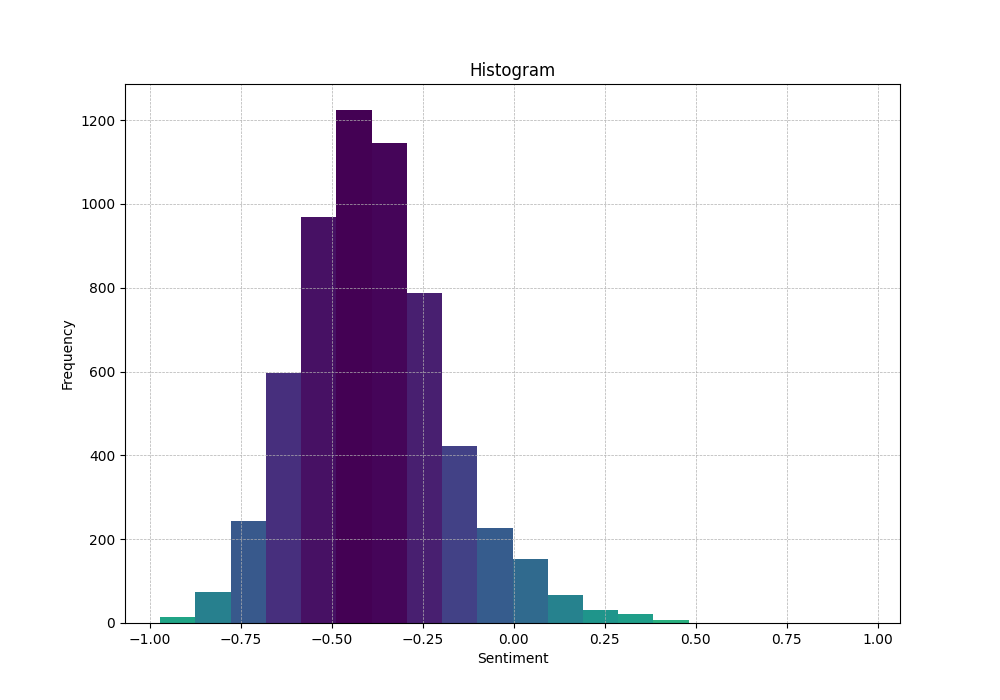
\includegraphics[width=\textwidth]{figures/sentiment_histogram.png}
    \caption[]{Lorem ipsum}
\end{figure}

\begin{figure}[!htb]
    \centering
    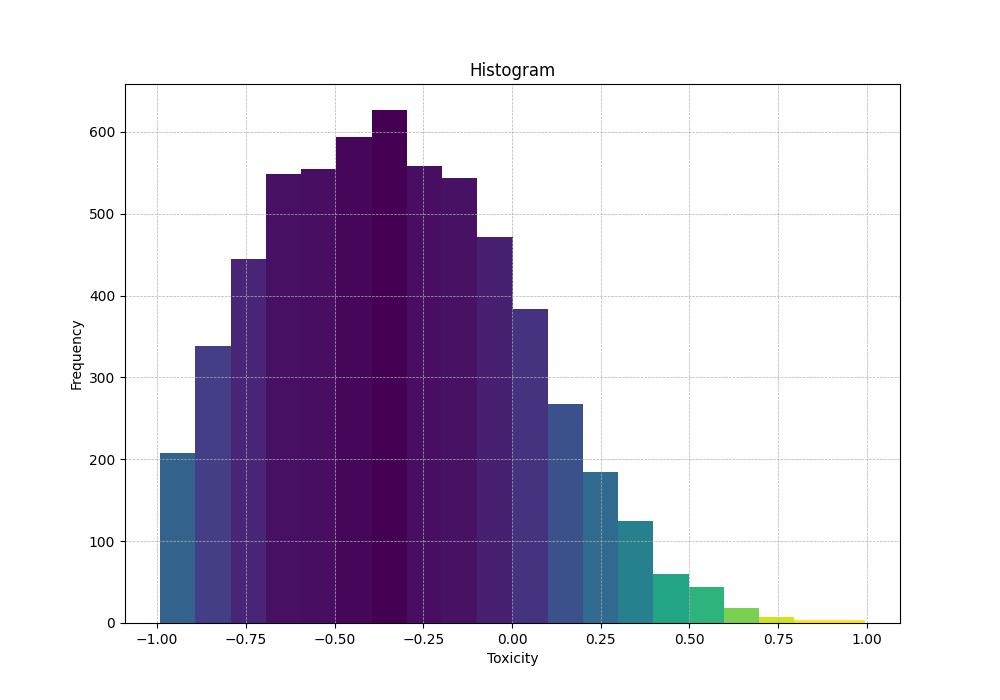
\includegraphics[width=\textwidth]{figures/toxicity_histogram.png}
    \caption[]{Lorem ipsum}
\end{figure}

\begin{figure}[!htb]
    \centering
    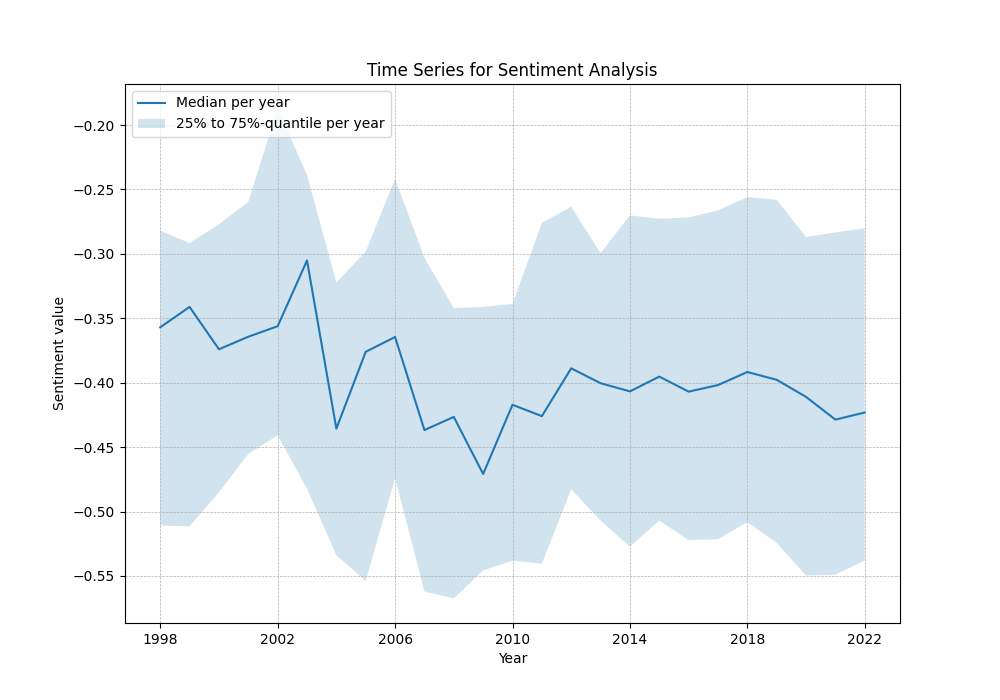
\includegraphics[width=\textwidth]{figures/time_series_sentiment.png}
    \caption[]{Lorem ipsum}
\end{figure}

\begin{figure}[!htb]
    \centering
    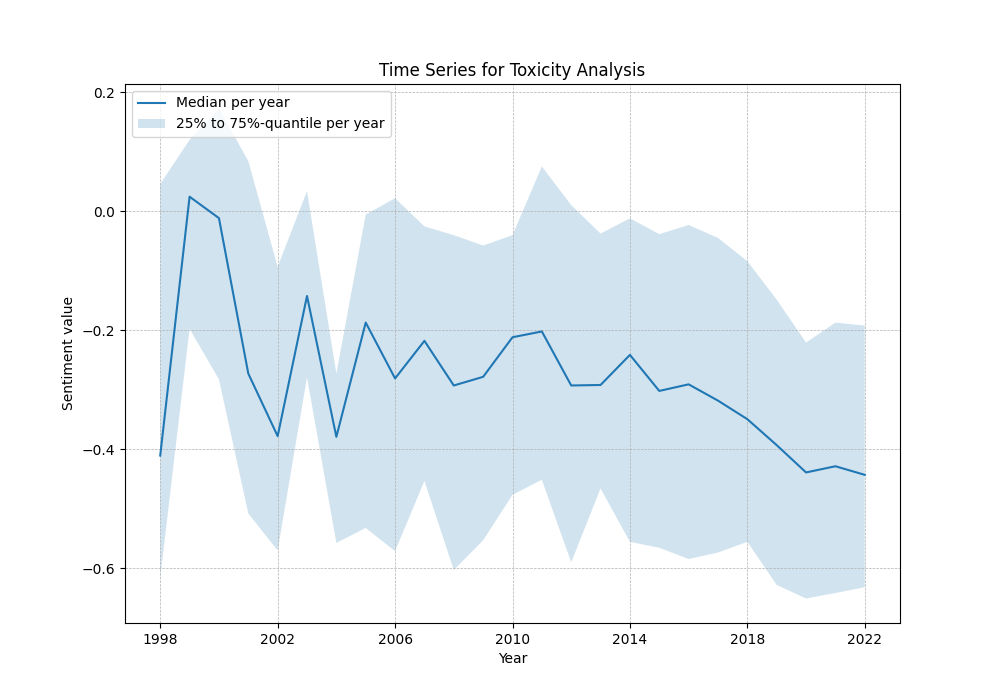
\includegraphics[width=\textwidth]{figures/time_series_toxicity.png}
    \caption[]{Lorem ipsum}
\end{figure}
